%\documentclass[11pt]{article}\usepackage{amssymb,amsmath,amsthm,hyperref,verbatim,pict2e,graphicx,array,listings,appendix,color}
\usepackage{algorithm,algorithmic,booktabs,marvosym,wrapfig,xytree,multicol,multirow,arydshln,nameref}
\hypersetup{colorlinks,citecolor=black,filecolor=black,linkcolor=black,urlcolor=black
	%pdfborderstyle={/S/U/W 1},urlbordercolor=1 0 0,linkbordercolor=.5 1 1, citebordercolor=.5 1 1
}
\usepackage[usenames]{xcolor} % color names ,dvipsnames,svgnames,table
\usepackage[utf8]{inputenc}
\usepackage[T1]{fontenc}
\usepackage[english]{babel}

% margins
\pagestyle{headings}
\oddsidemargin 0.0cm
\evensidemargin 0.0cm
\topmargin 0.0cm
\headheight 0.0cm
\headsep 1.0cm
\textheight 22.0cm
\textwidth 16.0cm
\parskip 0.1cm
\parindent 0.0cm
\footskip 1.0cm

% compact titles
\usepackage[compact]{titlesec}
\titlespacing{\section}{0pt}{8pt}{0pt}
\titlespacing{\subsection}{0pt}{8pt}{0pt}
\titlespacing{\subsubsection}{0pt}{8pt}{0pt}

% compact lists
\usepackage{enumitem}
\setitemize{noitemsep,topsep=0pt,parsep=0pt,partopsep=0pt}
\setenumerate{noitemsep,topsep=0pt,parsep=0pt,partopsep=0pt}
\def\ul{\begin{itemize}}
\def\ule{\end{itemize}}
\def\ol{\begin{enumerate}}
\def\ole{\end{enumerate}}

% misc
\def\up#1{\textsuperscript{#1}}
\def\quote#1{\par\begingroup\leftskip1em\rightskip\leftskip\textit{#1}\par\endgroup}


% listings
\definecolor{dkpink}{RGB}{200,0,100}
\definecolor{gray}{RGB}{128,128,128}
\lstset{
	xleftmargin=20pt,
	numberstyle=\tiny,stepnumber=1,numbersep=5pt,
	showstringspaces=true,         % underline spaces within strings
	tabsize=2,                      % sets default tabsize to 2 spaces
	captionpos=t,                   % sets the caption-position to bottom
	breaklines=true,                % sets automatic line breaking
	breakatwhitespace=true, % sets if automatic breaks should only happen at whitespace
	title=\lstname, % show the filename of files included with \lstinputlisting; also try caption instead of title
	basicstyle=\small\tt,keywordstyle=\color{blue},commentstyle=\color{gray},stringstyle=\color{dkpink}
}
% define Scala syntax
\lstdefinelanguage{Scala}{
	morekeywords={abstract,case,catch,class,def,do,else,extends,false,final,finally,for,if,implicit,import,%
	match,mixin,new,null,object,override,package,	private,protected,requires,return,sealed,super,this,%
	throw,trait,true,try,type,val,var,while,with,yield},
	otherkeywords={=>,<-,<\%,<:,>:,\#,@},sensitive=true,
	morecomment=[l]{//},	morecomment=[n]{/*}{*/},
	morestring=[b]",morestring=[b]',morestring=[b]"""
}

% title page
\makeatletter
\gdef\@subtitle{}\def\subtitle#1{\gdef\@subtitle{#1}}
\def\my@heading{
\def\ps@headings{\let\@mkboth\markboth
	\def\@evenhead{\small \rightmark \hfill \textit{\@title}, p.~\thepage}
	\def\@oddhead{\@evenhead}}\pagestyle{headings}}
\renewcommand{\maketitle}{
	%\begin{titlepage}
	\setcounter{page}{0}\thispagestyle{empty}
	{\centering\null\vfill
\includegraphics[width=5.5cm]{inc/logo_epfl.pdf} % EPFL logo
	\vspace{1.5cm}\hrule \vspace{2.5cm} {\LARGE \@title \par} {\large \emph \@subtitle \par}
	\vspace{2.75cm} {\Large \@author \par}
	\vspace{5.5cm} {\large School of Computer and Communication Sciences, EPFL \par}
	\vspace{1.0cm} {\@date \par} % date
	\vfill\null\par}\my@heading
	\newpage
	%\end{titlepage}
}
\newcommand{\shorttitle}{
	\thispagestyle{empty}
	\hfill 
\includegraphics[width=3cm]{inc/logo_epfl}\vspace{.1cm} % EPFL logo
	\begin{center} {\LARGE \@title} \\ \vspace{.1cm} {\large \textit{\@subtitle}} \\ \rule[1ex]{350pt}{.5pt} \\
	\@author \\ {\small School of Computer and Communication Sciences, EPFL} \vspace{.2cm} \\{\small \@date}
	\end{center} \vspace{.5cm}\my@heading
}
\makeatother

% new XeTeX title page
\usepackage[T1]{fontenc}
\usepackage{fontspec}
\newfontfamily\fonth{Helvetica}
\newfontfamily\fonthn{Helvetica Neue}
\newfontfamily\fonthc{Helvetica Neue Condensed Bold}
\newfontfamily\fonthl{Helvetica Neue UltraLight}

\makeatletter
\renewcommand{\maketitle}{
	%\begin{titlepage}
	\setcounter{page}{0}\thispagestyle{empty}
	\hfill 
\includegraphics[width=8.5cm]{inc/logo_epfl.pdf} \vfill
	{\fontsize{25pt}{11pt}\fonthc Master project report \vspace{0.5cm}} \\
	{\fontsize{40pt}{11pt}\fonthl \@title} \vspace{0.2cm} \\ {\fontsize{20pt}{11pt}\fonthl \@subtitle} \\
	\vspace{1.5cm} \\
	{\begin{tabular}{ll}
	Laboratory	& Programming Methods Laboratory, LAMP, EPFL \\
	Professor		& \href{mailto:martin.odersky@epfl.ch}{Martin Odersky} \\
	Supervisors	& \href{mailto:vojin.jovanovic@epfl.ch}{Vojin Jovanovic}, \href{mailto:manohar.jonnalagedda@epfl.ch}{Manohar Jonnalagedda}   \\
	Expert		& \href{mailto:mirco.dotta@typesafe.com}{Mirco Dotta}, Typesafe \\
	Student		& \href{mailto:thierry.coppey@epfl.ch}{Thierry Coppey} \\
	Semester		& Autumn 2012 \\
	\end{tabular}}
	\my@heading
	\newpage
	%\end{titlepage}
}
\makeatother

% appendix
\makeatletter
\let\origappendix\appendix
\renewcommand\appendix{\clearpage\pagenumbering{Roman}\origappendix\section*{\appendixname}\lstset{frame=tb,numbers=left}}
\makeatother

% default
\author{\href{mailto:thierry.coppey@epfl.ch}{Thierry Coppey}} %, \href{mailto:manohar.jonnalagedda@epfl.ch}{Manohar Jonnalagedda}, \href{mailto:nithin.george@epfl.ch}{Nithin George}
\begin{document}

\section{Benchmarks} \label{benchmarks}
In an attempt to provide realistic benchmarks, we tried to gather related implementations. The authors of \cite{gpu_atlp} did not respond to our multiple solicitations. The authors of \cite{swat_mega} were very friendly and provided us their source code. Unfortunately, since they address a different category of problem (they focus on huge serial problems whereas we focus on smaller non-serial problems) their implementation might be biased towards large sequences that our implementation cannot address. Finally, we asked lately the authors of \cite{gpu_rnafold} who did not respond either to our solicitations.

We organize the benchmarks as follow: if we have at our disposal a working implementation that could be run on our evaluation platform, we use it, otherwise, we refer to the related paper and rescale the result according to the memory throughput and computation throughput of the related device so that we can have a good approximation of how they could compare.

\subsection{Metrics} \label{metrics}
The main metrics of interest is the running time. In an attempt to reduce the variance, we would like to run multiple consecutive test and take the median running time, since the median is less sensitive to outlier than the average\cite{perfeval}. Unfortunately, several factors hampers these ideal conditions. First the variance in the running time of CUDA kernels might be significant, in particular for short running time. This is due to the fact that the GPU needs to be 'warmed-up' before actual computation can happen. Similarly, the JVM is also subject to running time variance that is mainly due to the garbage collection\footnote{\url{http://www.oracle.com/technetwork/java/javase/gc-tuning-6-140523.html\#cms.overhead}} and JIT optimizations \cite{java_jit}.

Also the input and problem might introduce variance. As example, we can consider two extreme cases: matrix chain multiplication and Zuker RNA folding, with a test environment of 100 random inputs (of length respectively 512 and 80) and a GPU warmup of 10 computations. In this settings, matrix chain multiplication computations are executed in a perfectly constant time\footnote{With respect to truncation and measurment accurcy, has less than 1\% of variation (not observable).} (0.127 seconds), which mean that we sufficiently reduced the noise. Oppositely, the Zuker RNA folding running times appear much more scattered as presented below:

\begin{figure}[H]\begin{center}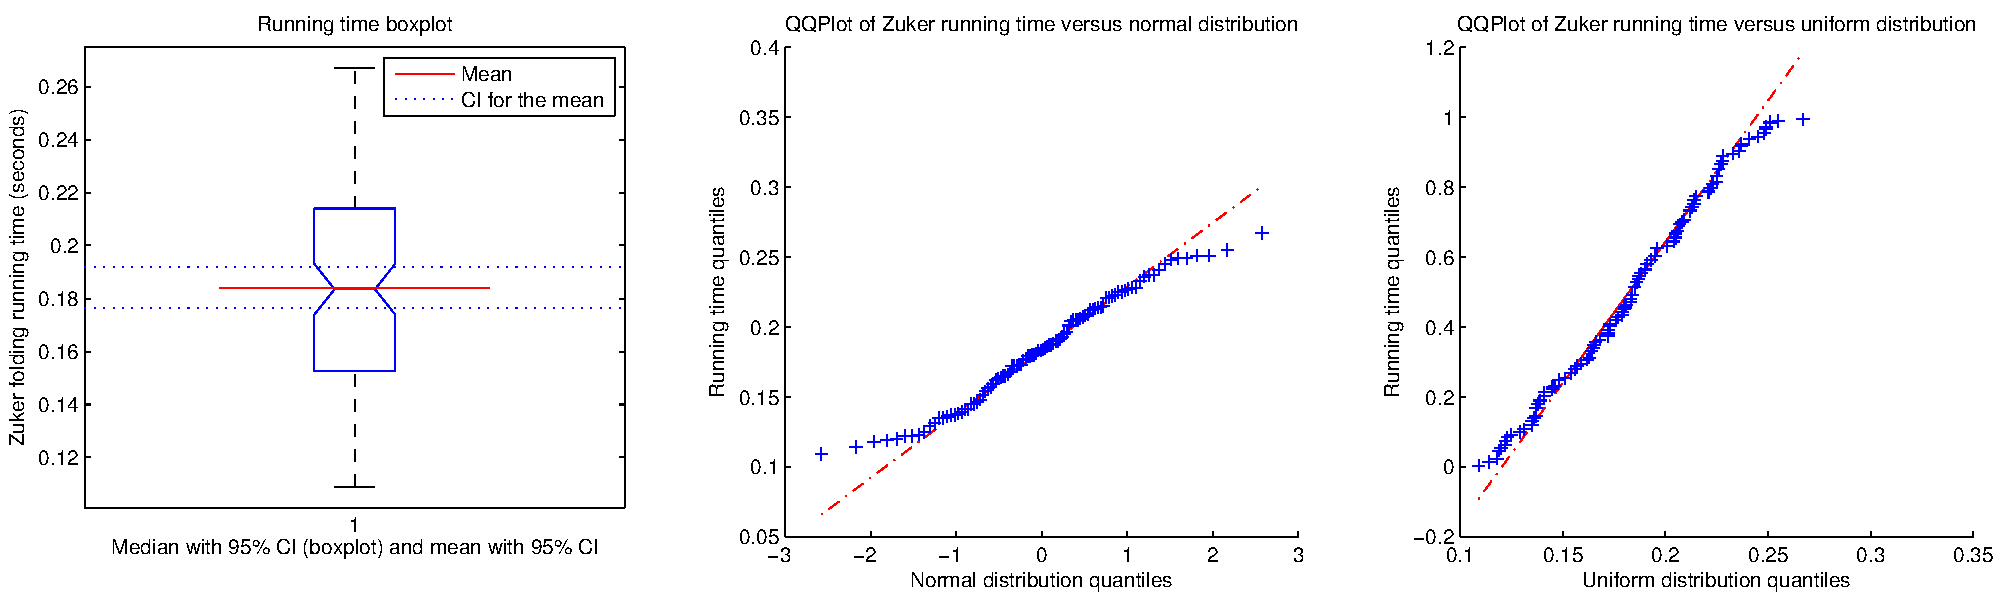
\includegraphics[width=16cm]{inc/var_zuker.pdf}\end{center}
\caption{Zuker folding running time (seconds). Quartiles: 0.152, 0.183 (median), 0.214}\label{fig:var_zuker}\end{figure}

Using the QQplot\footnote{Quantile-to-quantile plot, used to compare two distributions against each other.}, the distribution is heavily tailed (has more results towards the ends of the range) than a Gaussian distribution (fig.~\ref{fig:var_zuker} center) but fits better an uniform distribution (fig.~\ref{fig:var_zuker} right). If we run multiple time the program over the same input, we obtain the same behavior as with the matrix multiplication (strictly identical time); hence we can conclude that Zuker is an input sensitive problem whereas matrix chain multiplication is not. It follows that we need to be careful to test with exactly identical input set different implementations.

As the device memory is quite limited, it seems interesting to also take into account the space usage. The space requirement limits the maximal size of addressable problems  on a particular hardware. This might be a concern for large problems, because they would require special adaptation to handle such cases both correctly and efficiently. However, this metric heavily depends on the problem and simple solutions like using a device with larger memory or using main memory (if a $5\times$ slowdown is still acceptable) could solve this issue, hence we do not consider this metric hereafter (except as an upper bound on the dimension of the input).

\subsection{Benchmarking platform}
Our benchmarking platform is an Apple notebook with a Core i7-3720QM with 16Gb of main memory and an NVIDIA GeForce GT 650M running under MacOS X 10.8 and Oracle JDK 1.7.0-10. A workaround (see listing~\ref{cpu_workaround}) allows us to use the CPU to render the user interface while leaving the graphic card available to execute CUDA kernels. Unfortunately, due to impossibility to disable the watchdog timer in MacOS, CUDA kernels are limited to few seconds of running time before they are automatically aborted.

% ----------------------------------------------
\def\hh{\normalsize\bf}
\def\hl#1#2{\begin{minipage}{3.5cm} {\bf #1} \\[-2pt] \footnotesize #2 \vspace{6pt} \end{minipage}}
\def\hdps{\hl{DynaProg}{Scala parsers}}
\def\hdpc{\hl{DynaProg}{CUDA parsers}}
\def\hhoc{\hl{Optimized}{C, single thread}}
\def\hhog{\hl{Optimized}{CUDA, 64-bit}}
\def\hgapc{\hl{GAPC}{\cite{gapc_thesis}, C, single thread}}
\def\hatlp{\hl{ATLP}{\cite{gpu_atlp}, rescaled results$^{(1)}$}}
\def\hcua{\hl{CUDAlign}{\cite{swat_linear}, version 2.0}}

\def\hvien{\hl{ViennaRNA}{\cite{vienna_rna}}}
\def\hrna{\hl{RNAFold}{\cite{gpu_rnafold}}}

% ----------------------------------------------
% MatrixMult-512, Mac+JDK7
% -> Original: 24.658 sec
% -> Optimized concatenation: 18.924 sec
% -> Tabulation as arrays+inline: 14.849 sec
% -> Re-optimized concatenation: 10.76 sec
\newpage
\subsection{Matrix chain multiplication}
Since we have seen that this problem is not input sensitive in (\S\ref{metrics}), we can safely use different random number generators among different implementations without compromising the validity of the results.  Also note that the hand-optimized results are slightly worse than those presented in (\S\ref{baseline_impl}), this is caused by enabling the 64-bit mode. Since external libraries linked with the Java virtual machine must be in 64 bit, we also enabled this mode in hand-optimized version to maintain a fair comparison, thereby slightly reducing the performance of CUDA operations.
% CPU: DynaProg(Scala), hand optimized C, GAPC and ADPFusion
% GPU: GPU: DynaProg(CUDA), hand optimized CUDA, ATLP and GAPC-OpenCL?

\begin{table}[H]\begin{center}{\small\begin{tabular}{llrrrrrrr}\toprule
&\hh  Matrix dimension &\hh 64 &\hh 128 &\hh 192 &\hh 256 &\hh 384 &\hh 512 &\hh 768 \\
\midrule \multirow{4}{*}{\rotatebox{90}{\normalsize\bf CPU $\quad$}}
& \hdps	& 0.05	& 0.20	& 0.80	& 2.03	& 6.65	& 15.10	& 47.40	\\
& \hhoc	& <0.01	& <0.01	& <0.01	& 0.01	& 0.03	& 0.08	& 0.28	\\
& \hgapc	& 0.01	& 0.01	& 0.03	& 0.05	& 0.15	& 0.35	& 1.16	\\[-2pt]
\midrule \multirow{4}{*}{\rotatebox{90}{\normalsize\bf GPU $\quad$}}
& \hdpc	& 0.03	& 0.04	& 0.05	& 0.07	& 0.13	& 0.13	& 0.21	\\
& \hhog	& <0.01	& 0.01	& 0.01	& 0.02	& 0.04	& 0.08	& 0.17	\\
& \hatlp	& 0.17	&	 	&		& 0.20	& 		& 0.23	& 		\\
\midrule
&\hh Matrix dimension &\hh 1024 &\hh 1536 &\hh 2048 &\hh 3072 &\hh 4096 &\hh 6144 &\hh 8192 \\
\midrule \multirow{4}{*}{\rotatebox{90}{\normalsize\bf CPU $\quad$}}
& \hdps	& 109.77	& 368.21	& 877.30	& 3059.42 & 		& 		& 		\\
& \hhoc	& 1.18	& 7.06	& 19.81	& 78.90	& 206.56	& 799.53	& 2010.49 \\
& \hgapc	& 2.82	& 10.02	& 25.16	& 91.69	& 224.70	& 		&  		\\[-2pt]
\midrule \multirow{4}{*}{\rotatebox{90}{\normalsize\bf GPU $\quad$}}
& \hdpc	& 0.35	& 0.85	& 1.69	& 4.79	& 10.32	& 31.60	& 71.22	\\
& \hhog	& 0.32	& 0.82	& 1.65	& 4.74	& 10.35	& 31.94	& 72.38	\\
& \hatlp	& 0.40	& 0.74	& 1.33	& 3.43	& 7.29	& 		& 		\\
\bottomrule\end{tabular}}\end{center}\caption{Running time of matrix chain multiplication (in seconds)}\end{table}

$^{(1)}$ Assuming that 72\% of the running time is due to memory accesses, and considering a $3.55\times$ memory throughput slowdown of the original results (see \S\ref{results_discussion}). % 0.06 & 0.07 & 0.08 & 0.14 & 0.47 & 2.57 => f[x_] := (x*(1 - .72)) + (x*0.72)*(102.4/28.8)
% 0.1704 & 0.1988 & 0.2272 & .3976 & 1.3348 & 7.2988

The running time of DynaProg/CUDA includes the overhead of back and forth JNI conversion (scales linearly between 0.018 and 0.057 seconds) but does not include the overhead due to the code generation which decomposes in 0.068 seconds for analysis and code synthesis (once per algebra/grammar pair) and 0.086 + 1.753 seconds for respectively Scala and CUDA compilation (constant time, once per problem dimension). The results of the following problems are presented similarly.

For DynaProg/Scala we use a variant of the problem description: the original version only stores the matrix multiplication score whereas the modified version also stores the matrix dimension. This allows a speedup of $2.9\times$ probably due to the additional lookups overhead. Also with the default JVM parameters, the program cannot address sequences longer than $\sim 420$ elements due to a stack overflow, for these benchmarks, we increased this limit.

\subsection{Smith-Watermann}
% CPU: DynaProg(Scala), hand optimized C, GAPC and ADPFusion
% GPU: DynaProg(CUDA), hand optimized CUDA, CUDAlign
To maintain a fair comparison with other implementations, our algorithm needs to have the same complexity. Hence we use a variant of the Smith-Waterman algorithm: we encode our grammar in 3 tabulations as described in \S\ref{swat_affine}, whereas application like CUDAlign can leverage the domain-specific information that information of two of these matrices can be stored in the computation wavefront (see \S\ref{calc_simplifications}).

\begin{table}[H]\begin{center}{\small\begin{tabular}{llrrrrrrr}\toprule
&\hh  Matrix dimension &\hh 64 &\hh 128 &\hh 192 &\hh 256 &\hh 384 &\hh 512 &\hh 768 \\
\midrule \multirow{4}{*}{\rotatebox{90}{\normalsize\bf CPU $\quad$}}
& \hdps	& 0.04	& 0.13	& 0.27	& 0.48	& 1.07	& 1.92	& 4.33	\\
& \hhoc	& <0.01	& <0.01	& <0.01	& <0.01	& <0.01	& <0.01	& 0.01	\\
& \hgapc	& 0.01	& 0.01	& 0.01	& 0.01	& 0.02	& 0.03	& 0.06	\\[-2pt]
\midrule \multirow{4}{*}{\rotatebox{90}{\normalsize\bf GPU $\quad$}}
& \hdpc	& 0.03	& 0.03	& 0.03	& 0.04	& 0.05	& 0.05	& 0.06	\\
& \hhog	& 0.00	& 0.00	& 0.00	& 0.00	& 0.00	& 0.00	& 0.00	\\
& \hcua	& 0.11	& 0.12	& 0.07	& 0.07	& 0.07	& 0.07	& 0.13	\\
\midrule
&\hh Matrix dimension &\hh 1024 &\hh 1536 &\hh 2048 &\hh 3072 &\hh 4096 &\hh 6144 &\hh 8192 \\
\midrule \multirow{4}{*}{\rotatebox{90}{\normalsize\bf CPU $\quad$}}
& \hdps	& 7.84	& 18.95	& 33.63	& 70.86	& 		& 		& $^{(1)}\infty$ \\
& \hhoc	& 0.01	& 0.02	& 0.04	& 0.10	& 0.17	& 0.40	& 0.71	\\
& \hgapc	& 0.10	& 0.22	& 0.39	& 0.91	& 1.62	& 4.41	& 11.20 	\\[-2pt]
\midrule \multirow{4}{*}{\rotatebox{90}{\normalsize\bf GPU $\quad$}}
& \hdpc	& 0.07	& 0.11	& 0.15	& 0.13	& 0.20	& 0.32	& $^{(2)}$3.21 	\\
& \hhog	& 0.01	& 0.02	& 0.02	& 0.04	& 0.07	& 0.14	& 0.27	\\
& \hcua	& 0.13	& 0.15	& 0.14	& 0.14	& 0.15	& 0.17	& 0.20 	\\
\bottomrule\end{tabular}}\end{center}\caption{Running time of Smith-Waterman (in seconds)}\end{table}

$^{(1)}$ Extremely little progress due to intensive JVM garbage collection after some delay, even by tuning the JVM parameters ({\tt -Xss512m -Xmx12G -Xms12G}), and independently of whether top-down or bottom-up parsing approaches are taken. After a moment, most of the time is spent in (full) garbage collection. The aggregation function application contributes to approximately 30\% of the total running time.

$^{(2)}$ Since the memory requirements are larger than the device capacity, the backtrack matrix overflows in the main memory, thereby significantly degrading the performance. This extra memory requirement is due to the use of 3 matrices to avoid the non-serial dependencies (hence requiring at least $3 \cdot 2$ bytes of memory per matrix element for backtrack).

\subsection{Zuker RNA folding}
% CPU: DynaProg(Scala), GAPC, ADPFusion and ViennaRNA
% GPU: DynaProg(CUDA), RNAFold?/Lavenier VS ViennaRNA-OpenCL?, GAPC-OpenCL?

\begin{table}[H]\begin{center}{\small\begin{tabular}{llrrrrrrr}\toprule
&\hh  Matrix dimension &\hh 64 &\hh 128 &\hh 192 &\hh 256 &\hh 384 &\hh 512 &\hh 768 \\
\midrule \multirow{4}{*}{\rotatebox{90}{\normalsize\bf CPU $\quad$}}
& \hdps	& 0.07	& 0.67	& 2.26	& 4.98	& 17.61	& 39.44	& 130.71	\\
& \hvien	& 0.01	& 0.01	& 0.02	& 0.03	& 0.07	& 0.12	& 0.29	\\
& \hgapc	& 0.01	& 0.03	& 0.07	& 0.13	& 0.41	& 0.93	& 2.89	\\[-2pt]
\midrule \multirow{4}{*}{\vspace{12pt}\rotatebox{90}{\normalsize\bf GPU}}
& \hdpc	& 0.15	& 0.53	& 0.98	& 1.55	& 3.13	& 5.04	& 9.43	\\
& \hrna	& 0.06	& 0.11	& 0.14	& 0.20	& 0.44	& 0.80	& 1.89	\\
\midrule
&\hh Matrix dimension &\hh 1024 &\hh 1536 &\hh 2048 &\hh 3072 &\hh 4096 &\hh 6144 &\hh 8192 \\
\midrule \multirow{4}{*}{\rotatebox{90}{\normalsize\bf CPU $\quad$}}
& \hdps	& 306.12	& 1036.78 &		& 		& 		& 		& 	 	\\
& \hvien	& 0.57	& 1.53	& 3.19	& 9.37	& 20.18	& 59.65	& 133.65 	\\
& \hgapc	& 6.66	& 22.91	& 56.97	& 208.33	& 		& 		&  		\\[-2pt]
\midrule \multirow{4}{*}{\vspace{12pt}\rotatebox{90}{\normalsize\bf GPU}}
& \hdpc	& 15.10	& 33.62	& 61.76	& 166.84	& 393.76	& 		&  		\\
& \hrna	& 3.52	& 9.08	& 19.59	& 67.32	& 163.14	& 		& 		\\
\bottomrule\end{tabular}}\end{center}\caption{Running time of Zuker RNA folding (in seconds)}\end{table}

{\color{red} XXX: comment, explain energy coefficients, complexity, limit search space for bulges, algorithm variants and constraints RNAfold/Zuker}

% ------------------------------------------------------------------------------------------------
{\center\color{red} \noindent\rule{16cm}{0.4pt} \\ XXX: CONTINUE HERE :XXX \\}
% ------------------------------------------------------------------------------------------------

{\color{red}\ol
\item Write some conclusion ideas
\item use CUDA profiler(?)
\ole}

\subsection{Synthetical results}
XXX

{\color{red} We want to see the benefits of moving to CUDA, also compare to how far Scala is from C.}

RUN 5-10x until running time stabilizes on Scala

 {\color{red} Size analysis to know what storage size we require: ex: Zucker requires $O(n^2)+O(n)$ storage...}

XXX: future work: proper support of two-track grammars

XXX: future work, resize tables appropriately as in GAPL.

XXX: future work: infer automatically "always non-empty" property

{\color{red} XXX: say that Haskell package did not install and also time limited to provide largest result (but that are also less relevant as users do not want to wait)}

%\end{document}
